\documentclass[tikz,border=2mm]{standalone}
\usepackage{tikz}
\usetikzlibrary{arrows.meta,calc,positioning}
\definecolor{r2d}{HTML}{1F5A85}
\definecolor{local}{HTML}{B84537}
\definecolor{transfer}{HTML}{287C7B}
\definecolor{ink}{HTML}{263238}
\begin{document}
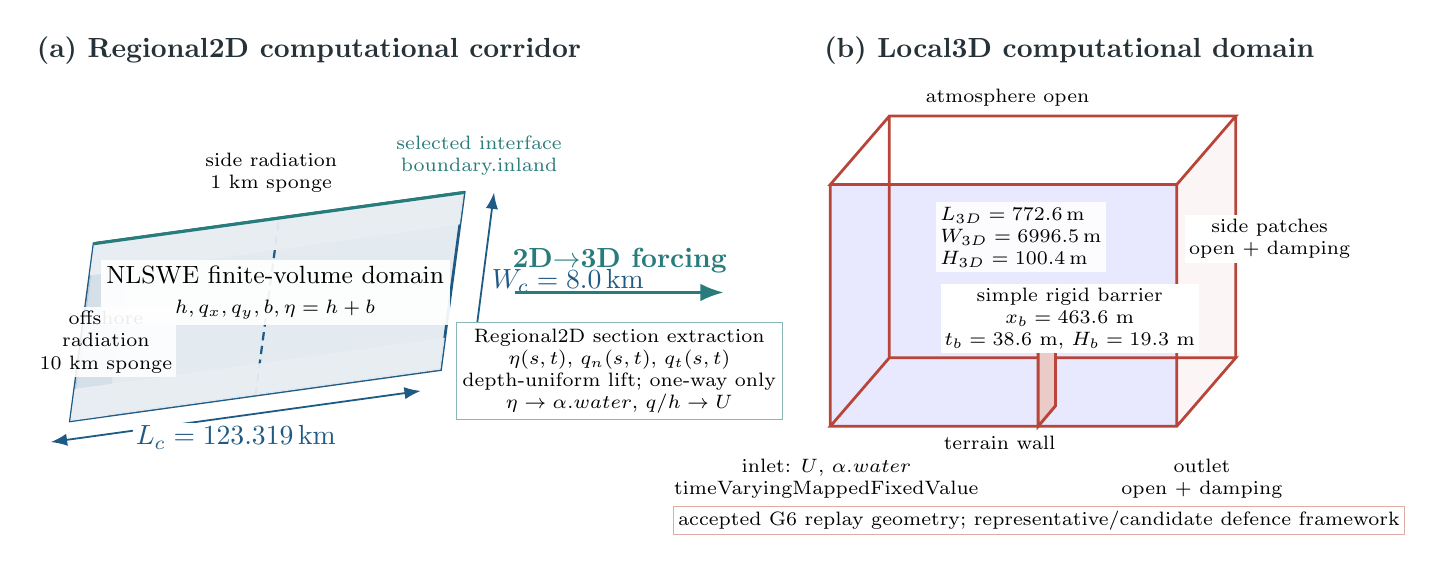
\begin{tikzpicture}[x=1cm,y=1cm,font=\sffamily,>=Latex]
\node[anchor=west,text=ink,font=\bfseries] at (0,6.15) {(a) Regional2D computational corridor};
\coordinate (A) at (0.55,1.45); \coordinate (B) at (5.25,2.10); \coordinate (C) at (5.55,4.35); \coordinate (D) at (0.85,3.70);
\path[fill=r2d!12] (A)--(B)--(C)--(D)--cycle;
\draw[r2d,line width=1pt] (A)--(B)--(C)--(D)--cycle;
\draw[r2d,densely dashed,line width=0.8pt] ($(A)!0.5!(B)$)--($(D)!0.5!(C)$);
\path[fill=r2d!20,opacity=0.85] (A)--($(A)!0.10!(B)$)--($(D)!0.10!(C)$)--(D)--cycle;
\path[fill=r2d!10,opacity=0.95] (A)--($(A)!0.18!(D)$)--($(B)!0.18!(C)$)--(B)--cycle;
\path[fill=r2d!10,opacity=0.95] ($(A)!0.82!(D)$)--(D)--(C)--($(B)!0.82!(C)$)--cycle;
\draw[transfer,line width=1.15pt] (D)--(C);
\node[align=center,font=\scriptsize,fill=white,inner sep=1pt,text=transfer] at (5.74,4.82) {selected interface\\boundary.inland};
\draw[<->,r2d,line width=0.65pt] (0.30,1.18)--(5.00,1.83) node[midway,below=2pt,fill=white,inner sep=1pt]{$L_c=123.319\,\mathrm{km}$};
\draw[<->,r2d,line width=0.65pt] (5.64,2.10)--(5.93,4.35) node[midway,right=2pt,fill=white,inner sep=1pt]{$W_c=8.0\,\mathrm{km}$};
\node[align=center,font=\scriptsize,fill=white,fill opacity=0.88,text opacity=1,inner sep=1.5pt] at (1.00,2.45) {offshore\\radiation\\$10$ km sponge};
\node[align=center,font=\scriptsize,fill=white,fill opacity=0.88,text opacity=1,inner sep=1.5pt] at (3.10,4.60) {side radiation\\$1$ km sponge};
% Lower side boundary uses the same radiation/sponge policy as the upper side boundary.
\node[align=center,font=\small,fill=white,fill opacity=0.92,text opacity=1,inner sep=2pt] at (3.15,3.08) {NLSWE finite-volume domain\\\scriptsize $h, q_x, q_y, b, \eta=h+b$};
\draw[-{Latex[length=3mm]},transfer,line width=1.2pt] (6.20,3.08)--(8.85,3.08) node[midway,above=3pt,text=transfer,font=\bfseries] {2D$\rightarrow$3D forcing};
\node[align=center,font=\scriptsize,fill=white,inner sep=2.2pt,draw=transfer!55,line width=0.45pt] at (7.52,2.08) {Regional2D section extraction\\$\eta(s,t)$, $q_n(s,t)$, $q_t(s,t)$\\depth-uniform lift; one-way only\\$\eta\rightarrow\alpha.water$, $q/h\rightarrow U$};
\node[anchor=west,text=ink,font=\bfseries] at (10.0,6.15) {(b) Local3D computational domain};
\coordinate (O) at (10.20,1.38); \coordinate (X) at (14.60,1.38); \coordinate (Y) at (15.35,2.25); \coordinate (OY) at (10.95,2.25);
\coordinate (Z) at (10.20,4.45); \coordinate (XZ) at (14.60,4.45); \coordinate (YZ) at (15.35,5.32); \coordinate (OYZ) at (10.95,5.32);
\path[fill=local!9] (O)--(X)--(Y)--(OY)--cycle;
\path[fill=blue!9] (O)--(X)--(XZ)--(Z)--cycle;
\path[fill=local!5] (X)--(Y)--(YZ)--(XZ)--cycle;
\draw[local,line width=1pt] (O)--(X)--(Y)--(OY)--cycle (Z)--(XZ)--(YZ)--(OYZ)--cycle (O)--(Z) (X)--(XZ) (Y)--(YZ) (OY)--(OYZ);
\coordinate (BX) at (12.840,1.38); \coordinate (BXY) at (13.060,1.64); \coordinate (BXZ) at (12.840,2.58); \coordinate (BXYZ) at (13.060,2.84);
\draw[local,line width=1.05pt,fill=local!28] (BX)--(BXY)--(BXYZ)--(BXZ)--cycle;
\node[font=\scriptsize,align=center,fill=white,inner sep=1.5pt] at (10.15,0.72) {inlet: $U$, $\alpha.water$\\timeVaryingMappedFixedValue};
\node[font=\scriptsize,align=center,fill=white,inner sep=1.5pt] at (14.92,0.72) {outlet\\open + damping};
\node[font=\scriptsize,align=center,fill=white,inner sep=1.5pt] at (15.78,3.76) {side patches\\open + damping};
\node[font=\scriptsize,align=center,fill=white,inner sep=1.5pt] at (12.45,5.55) {atmosphere open};
\node[font=\scriptsize,align=center,fill=white,inner sep=1.5pt] at (12.35,1.17) {terrain wall};
\node[font=\scriptsize,align=left,fill=white,fill opacity=0.9,text opacity=1,inner sep=1.7pt] at (12.62,3.78) {$L_{3D}=772.6\,\mathrm{m}$\\$W_{3D}=6996.5\,\mathrm{m}$\\$H_{3D}=100.4\,\mathrm{m}$};
\node[font=\scriptsize,align=center,fill=white,inner sep=1.4pt] at (13.240,2.75) {simple rigid barrier\\$x_b=463.6$ m\\$t_b=38.6$ m, $H_b=19.3$ m};
\node[font=\scriptsize,align=center,fill=white,draw=local!45,line width=0.4pt,inner sep=1.6pt] at (12.85,0.18) {accepted G6 replay geometry; representative/candidate defence framework};
\end{tikzpicture}
\end{document}
